\documentclass[12pt]{article}\usepackage[]{graphicx}\usepackage[]{color}
%% maxwidth is the original width if it is less than linewidth
%% otherwise use linewidth (to make sure the graphics do not exceed the margin)
\makeatletter
\def\maxwidth{ %
  \ifdim\Gin@nat@width>\linewidth
    \linewidth
  \else
    \Gin@nat@width
  \fi
}
\makeatother

\definecolor{fgcolor}{rgb}{0.345, 0.345, 0.345}
\newcommand{\hlnum}[1]{\textcolor[rgb]{0.686,0.059,0.569}{#1}}%
\newcommand{\hlstr}[1]{\textcolor[rgb]{0.192,0.494,0.8}{#1}}%
\newcommand{\hlcom}[1]{\textcolor[rgb]{0.678,0.584,0.686}{\textit{#1}}}%
\newcommand{\hlopt}[1]{\textcolor[rgb]{0,0,0}{#1}}%
\newcommand{\hlstd}[1]{\textcolor[rgb]{0.345,0.345,0.345}{#1}}%
\newcommand{\hlkwa}[1]{\textcolor[rgb]{0.161,0.373,0.58}{\textbf{#1}}}%
\newcommand{\hlkwb}[1]{\textcolor[rgb]{0.69,0.353,0.396}{#1}}%
\newcommand{\hlkwc}[1]{\textcolor[rgb]{0.333,0.667,0.333}{#1}}%
\newcommand{\hlkwd}[1]{\textcolor[rgb]{0.737,0.353,0.396}{\textbf{#1}}}%

\usepackage{framed}
\makeatletter
\newenvironment{kframe}{%
 \def\at@end@of@kframe{}%
 \ifinner\ifhmode%
  \def\at@end@of@kframe{\end{minipage}}%
  \begin{minipage}{\columnwidth}%
 \fi\fi%
 \def\FrameCommand##1{\hskip\@totalleftmargin \hskip-\fboxsep
 \colorbox{shadecolor}{##1}\hskip-\fboxsep
     % There is no \\@totalrightmargin, so:
     \hskip-\linewidth \hskip-\@totalleftmargin \hskip\columnwidth}%
 \MakeFramed {\advance\hsize-\width
   \@totalleftmargin\z@ \linewidth\hsize
   \@setminipage}}%
 {\par\unskip\endMakeFramed%
 \at@end@of@kframe}
\makeatother

\definecolor{shadecolor}{rgb}{.97, .97, .97}
\definecolor{messagecolor}{rgb}{0, 0, 0}
\definecolor{warningcolor}{rgb}{1, 0, 1}
\definecolor{errorcolor}{rgb}{1, 0, 0}
\newenvironment{knitrout}{}{} % an empty environment to be redefined in TeX

\usepackage{alltt}
\usepackage[margin=1in]{geometry}
\usepackage{natbib}
\usepackage{graphicx}
\usepackage{verbatim}
\usepackage{fancyhdr}
\usepackage{amsmath}
\usepackage{lscape}
\usepackage[colorlinks=true,citecolor=black,urlcolor=blue]{hyperref}
\setlength{\headheight}{15pt}

\title{Preliminary Analyses of New York Times Articles\\\large{Version 1}}
\author{Patrick Kraft}
\IfFileExists{upquote.sty}{\usepackage{upquote}}{}
\begin{document}

\maketitle



\section{Description of Dataset}

In order to analyze the content of the NYT articles using the structural topic model approach presented by \citet{roberts2014structural}, I transformed the scraped articles to a reduced dataset where each unique article is included as a \textit{single} observation. Articles that appeared several times in the original raw collection (e.g. most tweeted article for several days) or through different channels (e.g. most tweeted and most viewed) were combined in a single observation. Overall, the reduced dataset contains 5592 \textit{unique} articles for subsequent analyses.

For each observation, I created a vector of dichotomous variables indicating whether the respective article was included in each of the categories (emailed, facebook, etc.) at least once. Here is a sample of observations from this reduced dataset (article body and keywords are omitted).

\begin{knitrout}
\definecolor{shadecolor}{rgb}{0.969, 0.969, 0.969}\color{fgcolor}\begin{kframe}
\begin{verbatim}
##         id              title emailed facebook front tweeted viewed
## 23  100023    The Obama Years       1        0     0       0      1
## 50  100050  Complete Coverage       0        0     0       0      1
## 55  100055 Who Loves America?       1        1     0       1      1
## 74  100074 ISIS Heads to Rome       1        1     0       1      1
## 89  100089    The Human Stain       1        1     0       1      1
## 101 100101    What Greece Won       0        0     0       1      1
##     digital
## 23        1
## 50        0
## 55        1
## 74        1
## 89        1
## 101       1
\end{verbatim}
\end{kframe}
\end{knitrout}

The dataset contains a unique id for each article which can be used in subsequent analyses to link the observations back to the full (raw) dataset including multiple instances for each article. The variables \texttt{emailed} through \texttt{digital} represent the matrix of covariates that will be used in order to model differences in topical prevalence in the collection of documents.


\section{Initial Results for 20 Topics}

In order to provide a first validation of the method, I estimated a structural topic model with 20 topics using the \texttt{stm} package in \texttt{R} \citep{roberts2014structural,roberts2014stm}. Depending on the specific research question, the number of topics can be increased in subsequent iterations in order to capture more fine-grained differences in article contents. The following output presents an overview of the extracted topics by displaying words that are highly associated with the respective topic (using highest probability, FREX, Lift, Score, see \citealt{roberts2014stm}). It should be noted that I used the spectral initialization implemented in the \texttt{stm} package in order to specify starting values for the subsequent model estimation. \citet[12-13]{roberts2014stm} discuss different alternatives to specify starting values and argue that in practice, the spectral initialization can be utilized successfully with vocabularies smaller than 10,000 entries. However, the vocabulary for the analyses of NYT articles has a size of 10268, so it might make sense to look at alternative strategies to specify starting values as well. However, I'll leave this issue for future iterations of the analyses.

\begin{knitrout}
\definecolor{shadecolor}{rgb}{0.969, 0.969, 0.969}\color{fgcolor}\begin{kframe}
\begin{verbatim}
## Topic 1 Top Words:
##  	 Highest Prob: republican, senat, clinton, democrat, presid, polit, campaign 
##  	 FREX: clinton, senat, republican, bush, candid, mrs, voter 
##  	 Lift: corasan, jindal, rappeport, rubio, caucus, chozick, firstdraft 
##  	 Score: keyston, republican, clinton, senat, obama, democrat, bush 
## Topic 2 Top Words:
##  	 Highest Prob: game, said, team, player, play, season, year 
##  	 FREX: player, tournament, basketbal, coach, game, leagu, athlet 
##  	 Lift: dugout, quarterfin, shortstop, calipari, kaminski, mcilroy, mickelson 
##  	 Score: clog, coach, yanke, tournament, player, spieth, playoff 
## Topic 3 Top Words:
##  	 Highest Prob: one, like, time, just, peopl, can, say 
##  	 FREX: didn, mother, father, rememb, wasn, tell, friend 
##  	 Lift: farmhous, reread, bellow, unbear, empathi, motherhood, imaginari 
##  	 Score: farmhous, book, father, mother, novel, write, writer 
## Topic 4 Top Words:
##  	 Highest Prob: health, patient, said, studi, medic, doctor, care 
##  	 FREX: cancer, patient, clinic, health, virus, doctor, diseas 
##  	 Lift: genom, cardiovascular, cholesterol, prey, discussionhow, dietari, oncologist 
##  	 Score: prey, patient, health, cancer, medic, diseas, virus 
## Topic 5 Top Words:
##  	 Highest Prob: art, museum, work, china, world, new, year 
##  	 FREX: museum, chines, beij, exhibit, kong, hong, galleri 
##  	 Lift: jonah, archaeologist, beij, artwork, warhol, whitney, archaeolog 
##  	 Score: jonah, museum, art, china, artist, chines, beij 
## Topic 6 Top Words:
##  	 Highest Prob: iran, said, state, israel, obama, unit, nuclear 
##  	 FREX: nuclear, netanyahu, israel, iran, isra, palestinian, iranian 
##  	 Lift: bibi, knesset, lausann, moniz, natanz, nuclear, plutonium 
##  	 Score: knesset, iran, netanyahu, nuclear, israel, iranian, isra 
## Topic 7 Top Words:
##  	 Highest Prob: year, percent, bank, compani, market, billion, will 
##  	 FREX: investor, tax, bank, wage, billion, fed, economi 
##  	 Lift: binyamin, eurozon, glacial, krugman, bernank, sharehold, buffett 
##  	 Score: glacial, billion, tax, investor, compani, greec, bank 
## Topic 8 Top Words:
##  	 Highest Prob: new, york, food, citi, cook, like, time 
##  	 FREX: chef, recip, chicken, sandwich, chees, meat, bread 
##  	 Lift: dough, teju, asparagus, bigcitybookclub, brais, broth, dismal 
##  	 Score: dismal, nytoday, chef, wine, recip, food, fish 
## Topic 9 Top Words:
##  	 Highest Prob: citi, hous, build, new, park, street, home 
##  	 FREX: bedroom, beach, properti, park, hotel, outdoor, tower 
##  	 Lift: bookend, nytrealest, realti, fireplac, townhous, terrac, skylin 
##  	 Score: bookend, bedroom, park, terrac, citi, acr, avenu 
## Topic 10 Top Words:
##  	 Highest Prob: compani, use, water, said, technolog, will, new 
##  	 FREX: googl, technolog, environment, softwar, comput, appl, app 
##  	 Lift: android, emiss, gase, tesla, straddl, samsung, sensor 
##  	 Score: straddl, compani, googl, app, appl, automak, drought 
## Topic 11 Top Words:
##  	 Highest Prob: show, fashion, design, look, dress, wear, week 
##  	 FREX: fashion, leather, fur, dress, skirt, runway, coat 
##  	 Lift: appendto, croptyp, embeddedslideshowtmag, fullscreenslideshow, insidefashionweek, jsonslideshowcallback, margiela 
##  	 Score: sonni, fashion, runway, insidefashionweek, dior, appendto, croptyp 
## Topic 12 Top Words:
##  	 Highest Prob: said, state, islam, govern, militari, american, attack 
##  	 FREX: iraqi, houthi, militia, afghanistan, islam, milit, ukrain 
##  	 Lift: aden, anbar, donetsk, militia, nemtsov, abdu, caliph 
##  	 Score: donetsk, islam, yemen, houthi, saudi, iraqi, shiit 
## Topic 13 Top Words:
##  	 Highest Prob: school, student, said, univers, colleg, citi, educ 
##  	 FREX: student, teacher, school, educ, colleg, campus, emanuel 
##  	 Lift: huang, emanuel, internship, negro, undergradu, student, tuition 
##  	 Score: huang, student, school, blasio, colleg, emanuel, mayor 
## Topic 14 Top Words:
##  	 Highest Prob: time, book, new, said, news, report, page 
##  	 FREX: cabl, comcast, broadcast, televis, hbo, stream, fox 
##  	 Lift: softer, roku, hassanmarch, robertsapril, artsbeat, adeel, comcast 
##  	 Score: softer, comcast, hbo, cabl, book, netflix, broadband 
## Topic 15 Top Words:
##  	 Highest Prob: said, polic, offic, prison, year, citi, investig 
##  	 FREX: polic, prison, arrest, ferguson, inmat, sentenc, crime 
##  	 Lift: inmat, taser, slager, turbul, tsarnaev, durst, dzhokhar 
##  	 Score: turbul, polic, durst, inmat, prosecutor, ferguson, slager 
## Topic 16 Top Words:
##  	 Highest Prob: said, pilot, peopl, crash, one, plane, day 
##  	 FREX: pilot, crash, plane, earthquak, lubitz, nepal, flight 
##  	 Lift: aftershock, cockpit, germanw, nepal, airbus, düsseldorf, katmandu 
##  	 Score: katmandu, lubitz, nepal, ebola, earthquak, cockpit, liberia 
## Topic 17 Top Words:
##  	 Highest Prob: read, women, learn, can, social, life, world 
##  	 FREX: women, discrimin, read, gender, wisdom, skill, moral 
##  	 Lift: errol, highfalutin, attain, bitti, itti, kleiner, dirgi 
##  	 Score: attain, read, women, disunion, pao, kleiner, discrimin 
## Topic 18 Top Words:
##  	 Highest Prob: film, play, music, show, new, movi, theater 
##  	 FREX: theater, broadway, song, actor, music, charact, film 
##  	 Lift: ballad, manohla, dargi, iñárritu, sturdi, theatergo, playhous 
##  	 Score: sturdi, film, broadway, music, theater, movi, comedi 
## Topic 19 Top Words:
##  	 Highest Prob: state, said, law, court, case, feder, rule 
##  	 FREX: legal, law, court, rule, feder, suprem, judg 
##  	 Lift: inaccur, solicitor, scalia, plaintiff, burwel, injunct, litig 
##  	 Score: inaccur, court, feder, law, justic, attorney, subsidi 
## Topic 20 Top Words:
##  	 Highest Prob: said, peopl, new, like, work, compani, want 
##  	 FREX: busi, custom, sell, card, owner, retail, partner 
##  	 Lift: extravag, airbnb, etsi, yoga, entrepreneur, starbuck, wallet 
##  	 Score: extravag, compani, said, retail, yoga, studio, custom
\end{verbatim}
\end{kframe}
\end{knitrout}

Overall, the extracted topics have high face validity in the context of newspaper articles. Some of them clearly focus on political issues, such as the US presidential race, whereas others represent other themes common in newspapers, such as art, media, sports, or health issues. Based on the high probability words that are strongly associated with each topic, we can assign descriptive labels for each of the extracted topics. I decided to label the topics in the following way: 
\begin{enumerate}
\item Presidential race
\item Sports
\item Books
\item Health
\item Art
\item Iran/Israel
\item Banking/Financial
\item New York/Food
\item Real Estate
\item Technology
\item Fashion
\item Terrorism/Iraq
\item Education
\item Media
\item Police
\item Plane Crash
\item Gender
\item Film/Shows
\item Legal/Court
\item Business
\end{enumerate}

We can also investigate how frequently each topic was mentioned in the articles. The following plot displays the proportions of each individual topic in the overall text body.

\begin{knitrout}
\definecolor{shadecolor}{rgb}{0.969, 0.969, 0.969}\color{fgcolor}
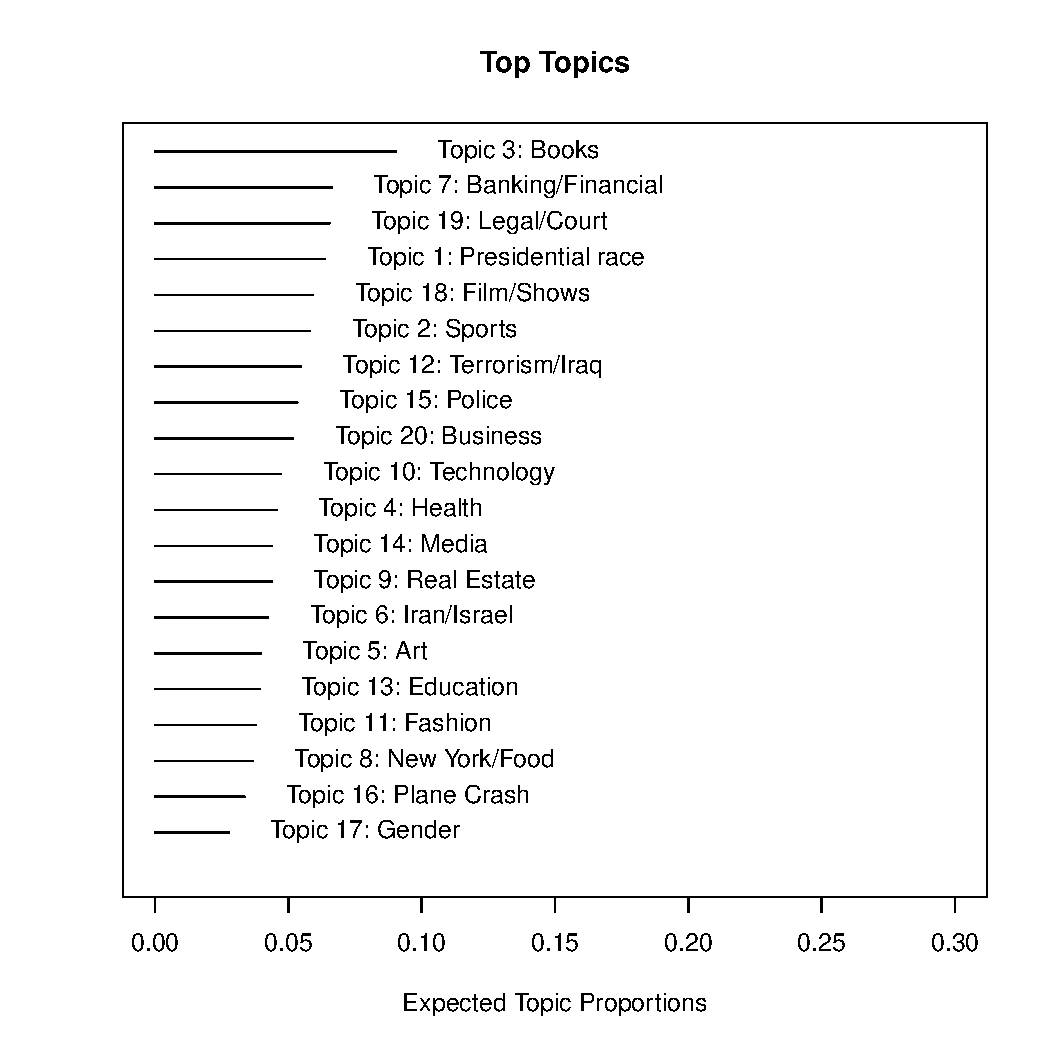
\includegraphics[width=\maxwidth]{figure/unnamed-chunk-4-1} 

\end{knitrout}

Interestingly, ``Books'' appears to be the most prevalent topic in the set of articles analyzed here. However, it should be kept in mind, that each observation in the document matrix can represent multiple instances of an article in the raw collection. The proportions presented here only describe the proportions in unique articles but does not take into account how often each of the articles was included originally (e.g. as most tweeted, or most viewed multiple times). 

We can also investigate the correlations between topics. Due to the fact that the structural topic model does not assume that each document has to be ascribed to a single topic but rather to a collection of topics, we can investigate the extent to which topics co-occur in documents. The following plot visualizes correlations between topics by linking topics that are correlated above a certain threshold (set at 0.01).

\begin{knitrout}
\definecolor{shadecolor}{rgb}{0.969, 0.969, 0.969}\color{fgcolor}
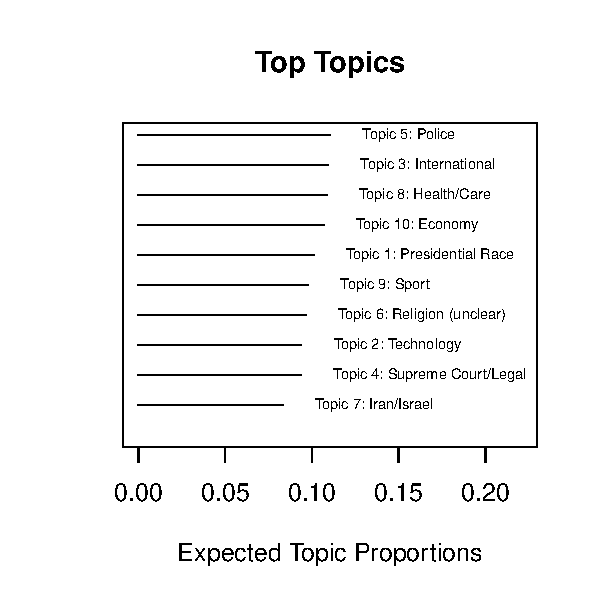
\includegraphics[width=\maxwidth]{figure/unnamed-chunk-5-1} 

\end{knitrout}

The connections between topics shows some interesting and plausible patterns. For example, it can be seen that the topics ``Fashion'', ``Art'', ``Film'', ``Books'', and ``Media'' cluster together or that ``Police'' is related to ``Legal/Court''. Overall, the results provide some additional validity for the topics extracted using the structural topic model.


\section{Differences in Topic Proportions between Categories}

As described in \citet{roberts2014structural}, the structural topic model not only extracts topics from a collection of documents but also allows us to directly model the prevalence of topics in specific documents based on a matrix of meta-covariates. While it is also possible to use covariates in order to model differences in words used to describe certain topics, we only focus on differences with regard to \textit{how much} a topic is discussed in specific articles.

The following figures display the change in the proportion to discuss each of the 20 topics for articles that were included in each of the categories or not.



\begin{knitrout}
\definecolor{shadecolor}{rgb}{0.969, 0.969, 0.969}\color{fgcolor}
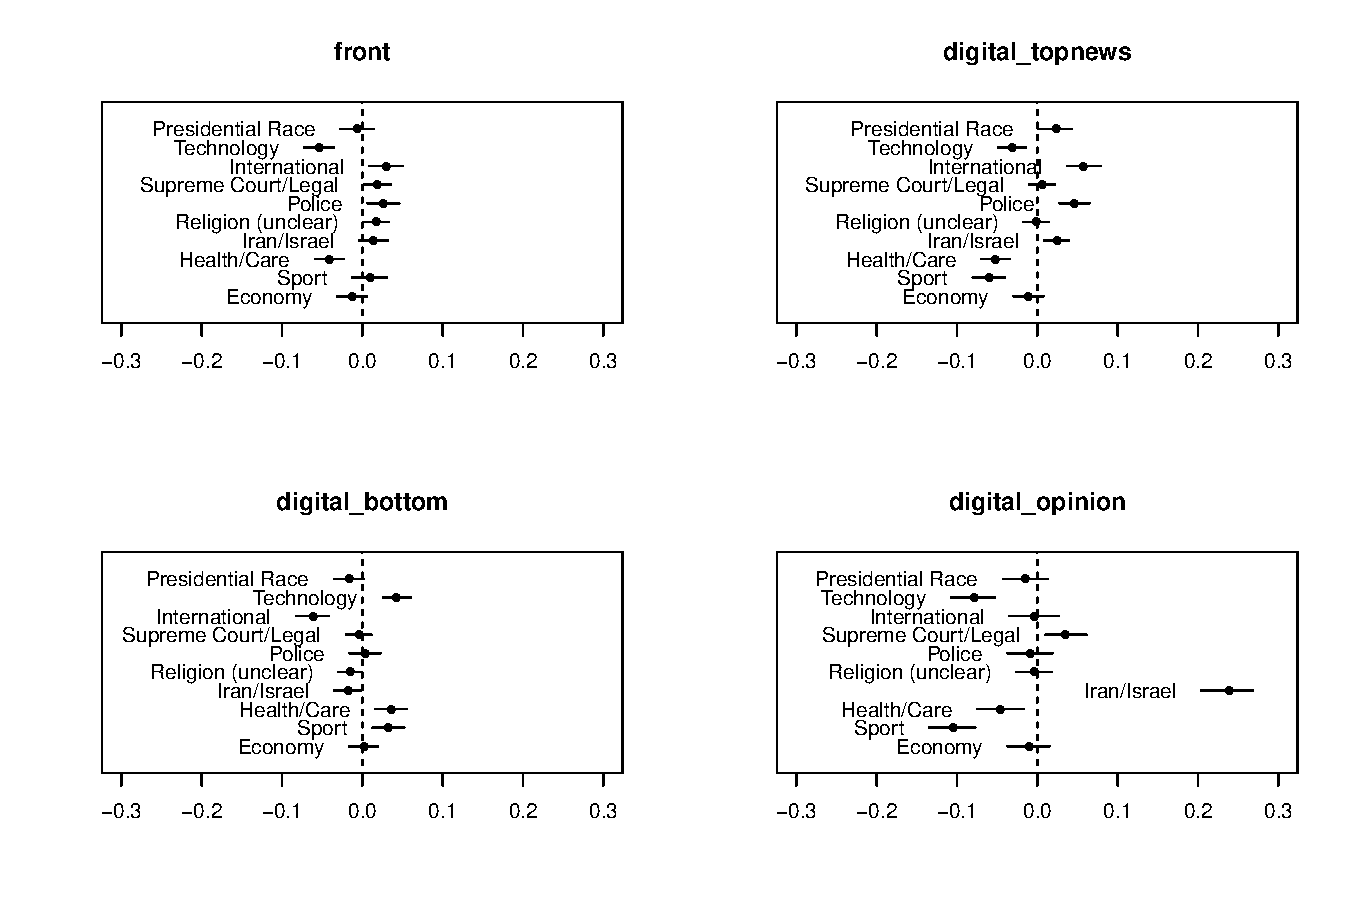
\includegraphics[width=\maxwidth]{figure/unnamed-chunk-7-1} 

\end{knitrout}
For articles that were most emailed, we see for example that the proportion to discuss the presidential race is significantly lower (as compared to articles that were not most emailed). On the other hand, articles that were most emailed included higher proportions of the ``Health'' topic.

\clearpage
\begin{knitrout}
\definecolor{shadecolor}{rgb}{0.969, 0.969, 0.969}\color{fgcolor}
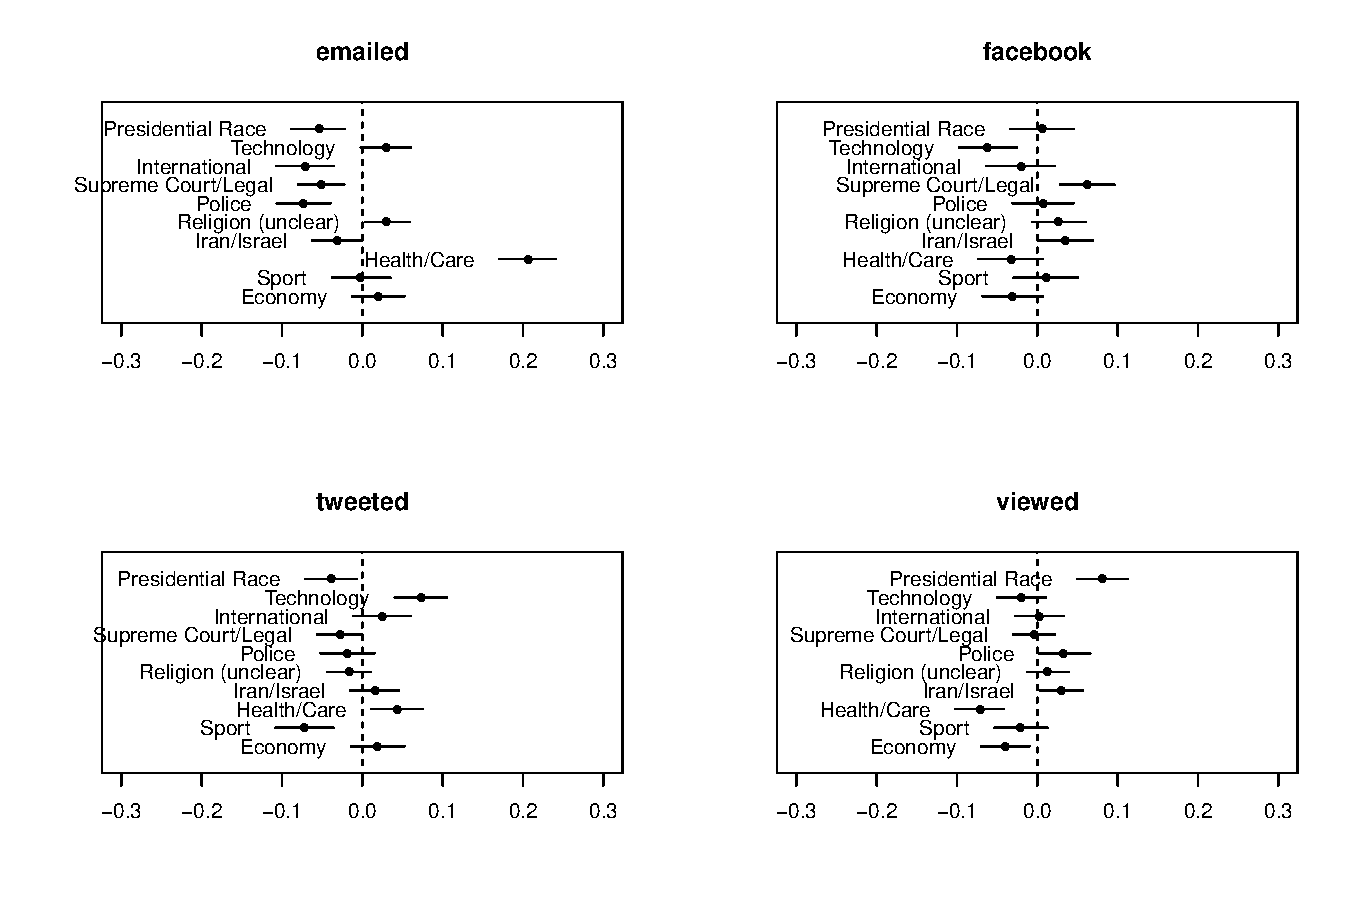
\includegraphics[width=\maxwidth]{figure/unnamed-chunk-8-1} 

\end{knitrout}
For articles that were most shared on facebook, there are hardly any significant differences with regard to the proportions of either of the 20 topics. Only the proportion of ``Business'' topics appears to be significantly lower in articles that were shared on facebook as compared to articles that were not shared on facebook.

\clearpage
\begin{knitrout}
\definecolor{shadecolor}{rgb}{0.969, 0.969, 0.969}\color{fgcolor}
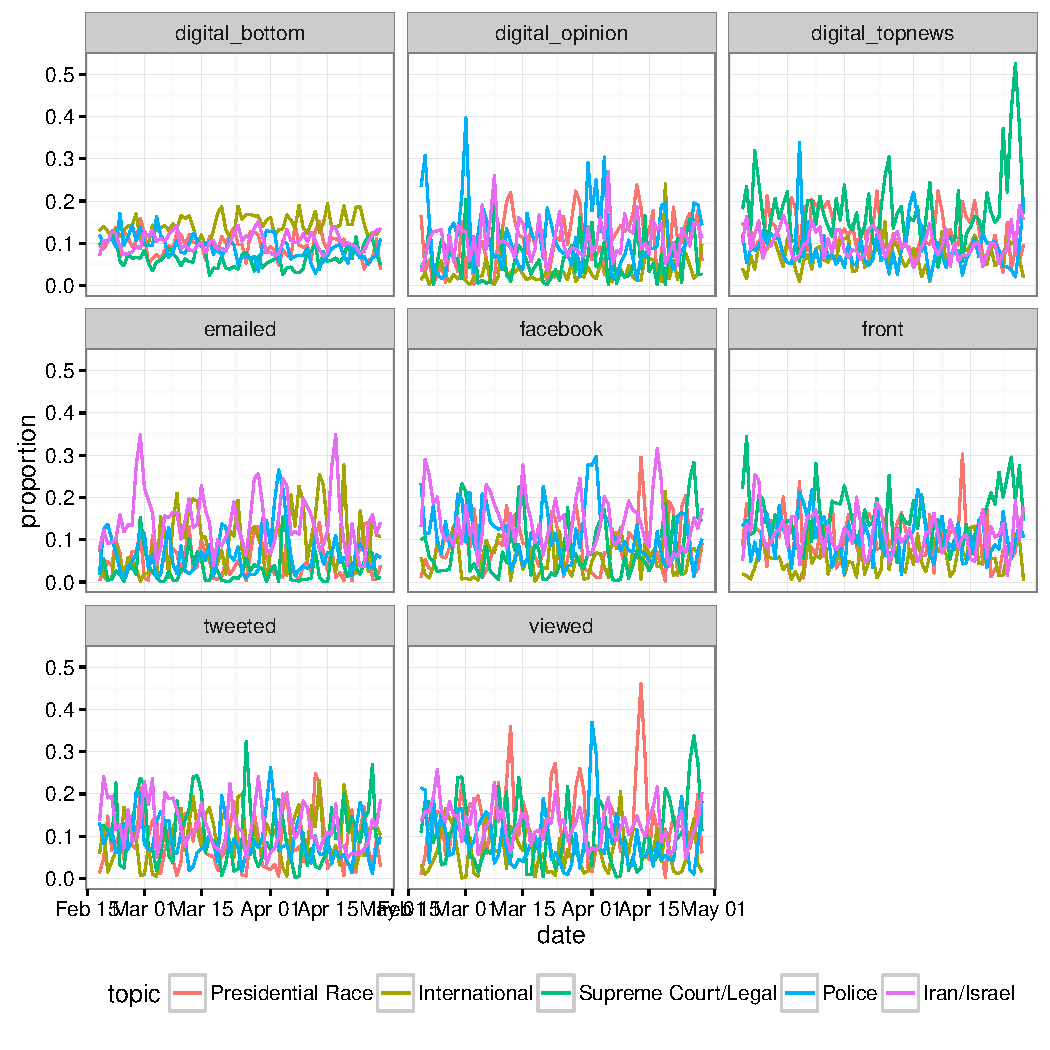
\includegraphics[width=\maxwidth]{figure/unnamed-chunk-9-1} 

\end{knitrout}
Looking at the topic proportions for front page articles, we can again observe several significant differences. For example, front page articles included higher proportions of political issues (presidential race, Iran/Israel, Terrorism/Iraq) and lower proportions of fashion, media, literature, and related topics. This result provides some additional validity for the model results.

\clearpage
\begin{knitrout}
\definecolor{shadecolor}{rgb}{0.969, 0.969, 0.969}\color{fgcolor}
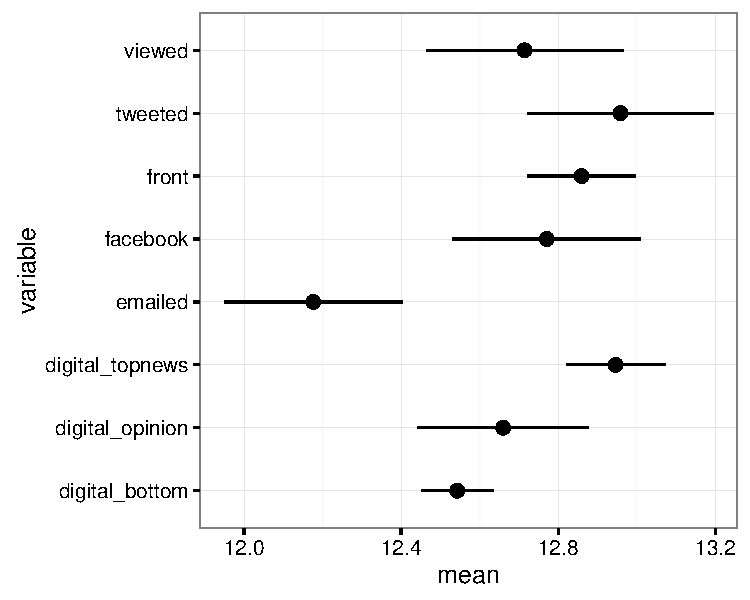
\includegraphics[width=\maxwidth]{figure/unnamed-chunk-10-1} 

\end{knitrout}
Articles that were most tweeted in the period under consideration encompass higher proportions of topics described as ``technology'', ``terrorism'', ``financial'', and ``health''. Interestingly, the proportion of ``sports'' is lower in tweeted articles as compared to the remaining articles.

\clearpage
\begin{knitrout}
\definecolor{shadecolor}{rgb}{0.969, 0.969, 0.969}\color{fgcolor}
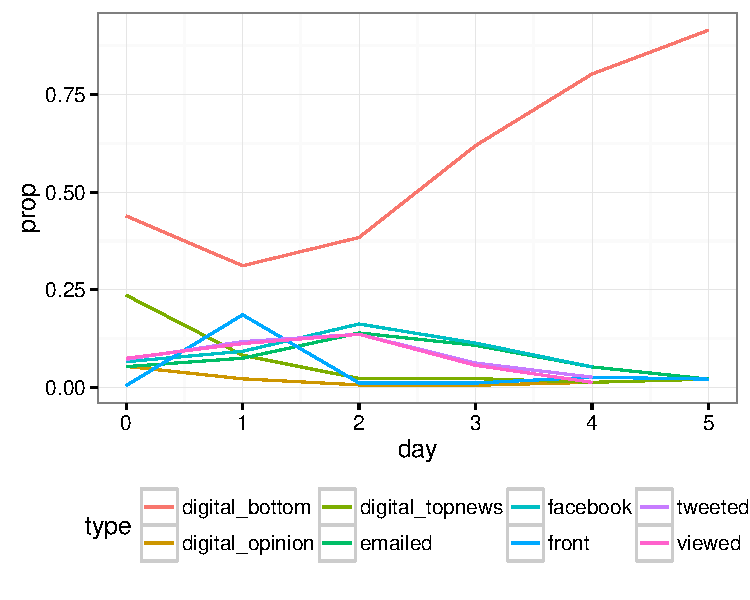
\includegraphics[width=\maxwidth]{figure/unnamed-chunk-11-1} 

\end{knitrout}
Looking at articles that were most viewed, we can see that the proportion of the topic ``presidential race'' is significantly larger. On the other hand, the proportion of ``health'', ``art'', or ``technology'' is lower in articles that were most viewed.

\clearpage
\begin{knitrout}
\definecolor{shadecolor}{rgb}{0.969, 0.969, 0.969}\color{fgcolor}
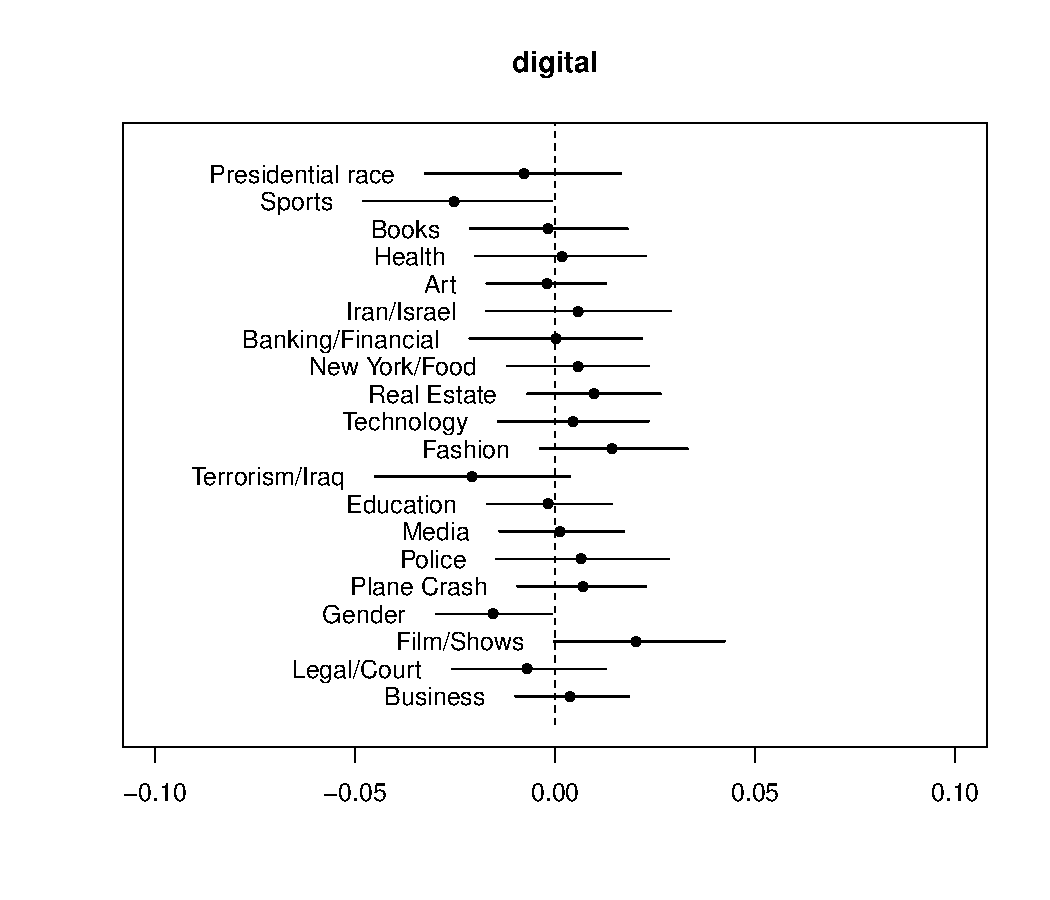
\includegraphics[width=\maxwidth]{figure/unnamed-chunk-12-1} 

\end{knitrout}
For articles that were included in the digital first page, no clear significant differences are observed. This could be due to the fact that most of the articles included in the analyses were part of the digital edition at some point (Only 4.99\% of the articles included in the analyses were not part of the digital edition.)

\clearpage
\section{Conclusion / Next Steps}
Overall, the structural topic model appears to recover plausible topics from the set of articles analyzed here. Subsequent iterations could investigate results for larger numbers of topics. Furthermore, additional analyses should be conducted in order to check robustness with regard to varying starting values. Other possible subsequent steps include:
\begin{itemize}
  \item investigate influence of other characteristics of articles (e.g. length of article)
  \item link topic model results back to full data, include information about persistence in different categories
  \item set up hazard model, explain how long a topic stays in the cycle
\end{itemize}


\bibliographystyle{/data/Copy/1-src/lit/apsr2006}
\bibliography{/data/Copy/1-src/lit/Literature}
\end{document}

